\section{Problema 3}
\begin{frame}{Contenido}
        \tableofcontents[sections={3}]
\end{frame}
\subsection{Presentación del problema}
    \begin{frame}{Presentación del problema}
        \begin{columns}
            \begin{column}{0.47\textwidth}
                Para la siguiente función:
                \[f(x,y)=x^{4}+y^{4}-x\]
    
            \begin{tikzpicture}
                \begin{axis}[
                samples=30,scale=0.75,hide axis]
                    \addplot3[surf, shader=interp]{H(\x,\y)};
                \end{axis}       
            \end{tikzpicture}
                
            \end{column}
            \begin{column}{0.47\textwidth}
                \justify
                Se pide:
                \begin{itemize}
                    \item Calcular el mínimo o mínimos de la función $f(x,y)$ de manera analítica.
                    \item Presentar y discutir el método numérico de newton para optimización y aplicarlo para encontrar los mínimos de $f(x,y)$
                    \item presentar y discutir un algoritmo genético para maximizar o minimizar funciones. Puede presentar su aplicación para el caso de una función de una variable.
                \end{itemize}
            \end{column}
        \end{columns}
                 
    \end{frame}
\subsection{Cálculo analítico de máximos y mínimos}
    \begin{frame}{Existencia de puntos críticos}
        \begin{columns}
            \begin{column}{0.47\textwidth}
                \justify
                \textbf{Cálculo de puntos máximos o mínimos de una función de dos variables.-}  Si buscamos los extremos relativos de una función hay que analizar los puntos donde las derivadas parciales valen cero o no existen. Dichos puntos se llaman puntos críticos o estacionarios de f.\footnotemark
            \end{column}
            \begin{column}{0.47\textwidth}
                Por lo tanto, hacemos:
                \[\frac{\partial f(x,y)}{\partial x}=f_{x}(x,y)=4x^{3}-1=0\]
                y:
                \[\frac{\partial f(x,y)}{\partial y}=f_{y}(x,y)=4y^{3}=0\]
                de donde obtenemos el punto crítico  $P(x_{0},y_{0})$ :
                \[x_{0}=\frac{\sqrt[3]{2}}{2} \approx 0.62996; 
                y_{0}=0\]
            \end{column}
        \end{columns}
        \footcitetext{Upm17}
    \end{frame}
    \begin{frame}[fragile,allowframebreaks]{Condiciones suficientes para la existencia de extremos relativos}
        \begin{columns}
            \begin{column}{0.47\textwidth}
                \justify
                \textbf{Criterio de la segunda derivada:}  
                \\Sea $z=f(x,y)$ una función definida en un espacio $D \subset R^{2}$ y $P(x_{0},y_{0}) \in D$. Supongamos que $f$ tiene derivadas parciales de primer y segundo orden continuas en $D$ y que $P(x_{0},y_{0})$ es un punto crítico de $f$, es decir $f_{x}(x_{0},y_{0})=0$ y $f_{y}(x_{0},y_{0})=0$, entonces se verifica que:
                \begin{enumerate}
                    \item $f$ tiene un punto máximo en $P(x_{0},y_{0})$ si:
                    \\
                    \scalebox{0.65}{%
                    $f_{xx}(x_{0},y_{0})<0$ y $\begin{vmatrix}
                     f_{xx}(x_{0},y_{0}) & f_{xy}(x_{0},y_{0})\\
                     f_{xy}(x_{0},y_{0}) & f_{yy}(x_{0},y_{0})
                    \end{vmatrix}>0$}
                    \setcounter{nameOfYourChoice}{\value{enumi}}
                \end{enumerate}
            \end{column}
            \begin{column}{0.47\textwidth}
                \begin{enumerate}
                    \setlength\itemsep{1em}
                    
                    \setcounter{enumi}{\value{nameOfYourChoice}}
                    \item $f$ tiene un punto mínimo en $P(x_{0},y_{0})$ si:
                    \\
                    \scalebox{0.65}{%
                    $f_{xx}(x_{0},y_{0})>0$ y $\begin{vmatrix}
                     f_{xx}(x_{0},y_{0}) & f_{xy}(x_{0},y_{0})\\
                     f_{xy}(x_{0},y_{0}) & f_{yy}(x_{0},y_{0})
                    \end{vmatrix}>0$}
                    
                    \item $f$ no tiene ni máximo ni mínimo en $P(x_{0},y_{0})$, es decir presente un punto silla sí:
                    \\
                    \centering{
                    \scalebox{0.65}{%
                    $\begin{vmatrix}
                     f_{xx}(x_{0},y_{0}) & f_{xy}(x_{0},y_{0})\\
                     f_{xy}(x_{0},y_{0}) & f_{yy}(x_{0},y_{0})
                    \end{vmatrix}<0$}}
                    
                    \item No podremos asegurar que $f$ tiene máximo ni mínimo si:
                    \\
                    \scalebox{0.65}{%
                     $\begin{vmatrix}
                     f_{xx}(x_{0},y_{0}) & f_{xy}(x_{0},y_{0})\\
                     f_{xy}(x_{0},y_{0}) & f_{yy}(x_{0},y_{0})
                    \end{vmatrix}=0$}
                \end{enumerate}
            \end{column}
\end{columns}       

\framebreak

\begin{columns}
    \begin{column}{0.47\textwidth}
                \justify
                Como vimos anteriormente, para calcular los máximos y mínimos de la ecuación $f(x,y)$ debemos calcular las segundas derivadas $f_{xx}(x,y)$, $f_{xy}(x,y)$ y $f_{yy}(x,y)$, y evaluarlas en el punto crítico $P(x_{0},y_{0})=P(0.63;0)$ para poder ubicar al punto crítico dentro de uno de los 4 casos enumerados, para tal fin procedemos a hallar las derivadas en cuestión:
                \begin{itemize}

                    \item $f_{xx}(x,y)=12x^{2}$, entonces
                    \\$f_{xx}(x_{0},y_{0})=4.76$
                \end{itemize}
                    
            \end{column}
            \begin{column}{0.47\textwidth}
                \begin{itemize}
                    \setlength\itemsep{1em}
                    \item $f_{xy}(x,y)=0$, entonces
                    \\$f_{xy}(x_{0},y_{0})=0$
                    
                    \item $f_{yy}(x,y)=12y^{2}$, entonces
                    \\$f_{yy}(x_{0},y_{0})=0$
                    \item Donde obtenemos que $f_{xx}(x_{0},y_{0})>0$, pero $\begin{vmatrix}
                     f_{xx}(x_{0},y_{0}) & f_{xy}(x_{0},y_{0})\\
                     f_{xy}(x_{0},y_{0}) & f_{yy}(x_{0},y_{0})
                    \end{vmatrix}=0$, por lo tanto, el punto podría ser un mínimo, pero el criterio del Hessiano no es concluyente.
            \end{itemize}
         \end{column}
\end{columns}        
    \end{frame}
    \begin{frame}[fragile,allowframebreaks]{Análisis del entorno}
        \begin{columns}
    \begin{column}{0.47\textwidth}
        \begin{itemize}
            \item Analizamos la función $f(x,y)$ en $\color{blue}P(x_{0},y_{0})=P(0.63;0)$, y obtenemos:
                    \\
                    $\color{blue}f(x_{0},y_{0})=-0.47247$
            \item Analizamos la función $f(x,y)$ en $P_{1,2}(x_{0}-0.1,y_{0} \pm 0.1)=P_{1,2}(0.53; \pm 0.1)$, y obtenemos:
                    \\
                    $f(x_{0}-0.1,y_{0} \pm 0.1)=-0.45$
            \item De lo analizado podemos observar que $P$ es un punto más bajo que $P_{1,2}$, podemos afirmar parcialmente que $P$ es punto mínimo de la función $f$.
        \end{itemize}
    \end{column}
    \begin{column}{0.47\textwidth}
        Analizamos en el plano $x=x_{0}$:
        \begin{tikzpicture}[samples=50]
            \begin{axis}[
                samples=30,axis lines=middle, axis on top, 
                view={60}{45},  
                xmin=-1,
                xmax=1,
                ymin=-1,
                ymax=1,       
                miter limit=1,scale=0.75]
                
                \addplot3[ smooth,     
                    surf,
                    faceted color=gray,
                    line width=0.0001pt, 
                    fill=white, 
                    domain=-1:0.62996,
                    y domain = -1:1,
                    samples = 20,
                    samples y = 20]
                    {H(\x,\y)};
                    
                \addplot3[y domain=-1:1,
                    samples y = 50, samples= 0, red, thick] 
                    ({0.62996},{y},{H(0.62996,y)});
                    
                \addplot3[y domain=-.1:.1,
                    samples y = 10, samples= 0, blue, thick] 
                    ({0.52996},{y},{H(0.52996,y)});
                \addplot3[domain=0.52996:0.62996,
                    samples = 10, samples y = 0, blue, thick] 
                    ({x},{0.1},{H(x,0.1)});  
                    
                \addplot3[domain=0.52996:0.62996,
                    samples = 10, samples y = 0, blue, thick] 
                    ({x},{-0.1},{H(x,-0.1)});  
                
            \end{axis}
            
        \end{tikzpicture} 
    \end{column}
    
\end{columns}

\framebreak

\begin{columns}
    \begin{column}{0.47\textwidth}
        Analizamos en el plano $y=y_{0}$:
        \begin{tikzpicture}[samples=50]
            \begin{axis}[
                samples=30,axis lines=middle, axis on top, 
                view={310}{50},  
                xmin=-0.4,
                xmax=1.6,
                ymin=-1,
                ymax=1,       
                miter limit=1,scale=0.75]
                
                \addplot3[ smooth,     
                    surf,
                    faceted color=gray,
                    line width=0.0001pt, 
                    fill=white, 
                    domain=-0.4:0.62996,
                    y domain = 0:1,
                    samples = 10,
                    samples y = 10]
                    {H(\x,\y)};
                \addplot3[ smooth,     
                    surf,
                    faceted color=gray,
                    line width=0.0001pt, 
                    fill=white, 
                    domain=0.62996:1.5,
                    y domain = -1:1,
                    samples = 10,
                    samples y = 19]
                    {H(\x,\y)};
                    
                \addplot3[domain=-0.4:1.5,
                    samples y = 0, samples= 50, red, thick] 
                    ({x},{0},{H(x,0)});
                    
                \addplot3[y domain=-.1:.1,
                    samples y = 10, samples= 0, blue, thick] 
                    ({0.72996},{y},{H(0.72996,y)});
                \addplot3[y domain=0:.1,
                    samples y = 10, samples= 0, blue, thick] 
                    ({0.52996},{y},{H(0.52996,y)});
                \addplot3[domain=0.52996:0.72996,
                    samples = 10, samples y = 0, blue, thick] 
                    ({x},{0.1},{H(x,0.1)});  
                    
                \addplot3[domain=0.62996:0.72996,
                    samples = 10, samples y = 0, blue, thick] 
                    ({x},{-0.1},{H(x,-0.1)});  
                
            \end{axis}
            
        \end{tikzpicture} 
    \end{column}
    \begin{column}{0.47\textwidth}
        \begin{itemize}
            \item Recordando que el punto $\color{blue}P(x_{0},y_{0})=P(0.63;0)$ en la función $f(x,y)$ toma el valor de:
                    \\
                    $\color{blue}f(x_{0},y_{0})=-0.47247$
            \item Analizamos la función $f(x,y)$ en $P_{3,4}(x_{0}+0.1,y_{0} \pm 0.1)=P_{3,4}(0.73; \pm 0.1)$, y obtenemos:
                    \\
                    $f(x_{0}+0.1,y_{0} \pm 0.1)=-0.446$
            \item De lo analizado podemos observar que $P$ es un punto más bajo que $P_{1,2,3,4}$, podemos afirmar que $P$ es punto mínimo de la función $f$.
        \end{itemize}
    \end{column}
\end{columns}


    


    \end{frame}
\subsection{Resolución por el ``Método de Newton''}
\begin{frame}[fragile,allowframebreaks]{Método de Newton}
    \justify
Para aproximarnos a un punto mínimo en la función $f$ a través del método de Newton asumimos un valor donde esperamos que exista un punto mínimo, por ejemplo para nuestro caso usaremos el punto $K(x_{k},y_{k})=(0.5,0.5)$ entonces calculamos un punto más próximo al mínimo esperado al que llamaremos $K+1$, con la siguiente expresión:
\[X_{K+1}=X_{K}-H^{-1}_{f}(X_{K}) * \nabla f(X_{K}) \]
\flushleft
donde:
\begin{itemize}
    \item $X_{K}$: es el punto $K$ expresado vectorialmente, es decir, en nuestro caso $X_{K}=\begin{bmatrix}
        x_{k} \\
        y_{k}
    \end{bmatrix}=
    \begin{bmatrix}
        0.5 \\
        0.5
    \end{bmatrix}$.
    \item $H^{-1}_{f}(X_{K})$: es  la inversa del Hessiano de la función $f$ evaluada en el punto $K$.
    \item $\nabla f(X_{K})$: es la gradiente de la función $f$ evaluada en el punto $K$.
\end{itemize}

\framebreak

cómo vimos anteriormente el hessiano de la funcion $f$, está definido por:
\[H_{f}=\begin{bmatrix}
  f_{xx}(x,y) & f_{xy}(x,y)\\
 f_{xy}(x,y) & f_{yy}(x,y)
\end{bmatrix}=
\begin{bmatrix}
  12x^{2} & 0\\
 0 & 12y^{2}
\end{bmatrix}\]
y la gradiente no es mas qué:
\[\nabla f(X) = \begin{bmatrix}
    f_{x}(x,y)\\
    f_{y}(x,y)
\end{bmatrix}
=\begin{bmatrix}
    4x^{3}-1\\
    4y^{3}
\end{bmatrix}\]
Es decir calcularemos, para nuestro caso particular:
\[X_{K+1}=\begin{bmatrix}
        x_{k} \\
        y_{k}
    \end{bmatrix}-\begin{bmatrix}
  12x^{2} & 0\\
 0 & 12y^{2}
\end{bmatrix}^{-1} * \begin{bmatrix}
    4x^{3}-1\\
    4y^{3}
\end{bmatrix}\]

\framebreak

\begin{itemize}
    \item Realizamos la {\color{blue}primeraa iteración} haciendo $
    \begin{bmatrix}
        x_{k} \\
        y_{k}
    \end{bmatrix}=
    \begin{bmatrix}
        0.5 \\
        0.5
    \end{bmatrix}$, de donde obtenemos:\\
    \scalebox{0.75}{$X_{K+1}=\begin{bmatrix}
        0.5 \\
        0.5
    \end{bmatrix}-\begin{bmatrix}
  12(0.5)^{2} & 0\\
 0 & 12(0.5)^{2}
\end{bmatrix}^{-1} * \begin{bmatrix}
    4(0.5)^{3}-1\\
    4(0.5)^{3}
\end{bmatrix}=\begin{bmatrix}
        0.6666\\
        0.3333
\end{bmatrix}
$}
\item Realizamos la {\color{blue}segunda iteración} haciendo $
    \begin{bmatrix}
        x_{k} \\
        y_{k}
    \end{bmatrix}=
    \begin{bmatrix}
        0.666 \\
        0.333
    \end{bmatrix}$, de donde obtenemos:\\
    \scalebox{0.75}{$X_{K+1}=\begin{bmatrix}
        0.666 \\
        0.3333
    \end{bmatrix}-\begin{bmatrix}
  12(0.666)^{2} & 0\\
 0 & 12(0.333)^{2}
\end{bmatrix}^{-1} * \begin{bmatrix}
    4(0.666)^{3}-1\\
    4(0.333)^{3}
\end{bmatrix}=\begin{bmatrix}
        0.6319\\
        0.2222
\end{bmatrix}
$}
\item Realizamos la {\color{blue}tercera iteración} haciendo $
    \begin{bmatrix}
        x_{k} \\
        y_{k}
    \end{bmatrix}=
    \begin{bmatrix}
        0.6319 \\
        0.2222
    \end{bmatrix}$, de donde obtenemos:\\
    \scalebox{0.75}{$X_{K+1}=\begin{bmatrix}
        0.6319 \\
        0.2222
    \end{bmatrix}-\begin{bmatrix}
  12(0.6319)^{2} & 0\\
 0 & 12(0.2222)^{2}
\end{bmatrix}^{-1} * \begin{bmatrix}
    4(0.6319)^{3}-1\\
    4(0.2222)^{3}
\end{bmatrix}=\begin{bmatrix}
        0.63\\
        0.1481
\end{bmatrix}
$}
\item Realizamos la {\color{blue}cuarta iteración} haciendo $
    \begin{bmatrix}
        x_{k} \\
        y_{k}
    \end{bmatrix}=
    \begin{bmatrix}
        0.63 \\
        0.1481
    \end{bmatrix}$, de donde obtenemos:\\
    \scalebox{0.75}{$X_{K+1}=\begin{bmatrix}
        0.63 \\
        0.1481
    \end{bmatrix}-\begin{bmatrix}
  12(0.63)^{2} & 0\\
 0 & 12(0.1481)^{2}
\end{bmatrix}^{-1} * \begin{bmatrix}
    4(0.63)^{3}-1\\
    4(0.1481)^{3}
\end{bmatrix}=\begin{bmatrix}
        0.63\\
        0.0987
\end{bmatrix}
$}
\item Realizamos la {\color{blue}quinta iteración} haciendo $
    \begin{bmatrix}
        x_{k} \\
        y_{k}
    \end{bmatrix}=
    \begin{bmatrix}
        0.63 \\
        0.0987
    \end{bmatrix}$, de donde obtenemos:\\
    \scalebox{0.75}{$X_{K+1}=\begin{bmatrix}
        0.63 \\
        0.0987
    \end{bmatrix}-\begin{bmatrix}
  12(0.63)^{2} & 0\\
 0 & 12(0.0987)^{2}
\end{bmatrix}^{-1} * \begin{bmatrix}
    4(0.63)^{3}-1\\
    4(0.0987)^{3}
\end{bmatrix}={\color{red}\begin{bmatrix}
        0.63\\
        0.0658
\end{bmatrix}
}$}
\end{itemize}
Como hemos visto, el método lleva a la convergencia del punto inicial elegido hacia el punto crítico que calculamos analíticamente.

\framebreak
Finalmente, para saber si el punto encontrado es un máximo o un mínimo local, tenemos que evaluar $f_{xx}$, al igual que en el método analítico, si $f_{xx}<0$, entonces estamos hablando de un máximo local, si, por el contrario $f_{xx}>0$, entonces el punto analizado es un mínimo local.
\end{frame}
\subsection{Resolución por ``algoritmo genético''}
\begin{frame}[fragile,allowframebreaks]{Resolución por algoritmos genéticos}
    Los algoritmos genéticos tienen cinco etapas
\begin{itemize}
    \item Definición de un individuo
    \item Creación de una población
    \item Medición del éxito de la población 
    \item Entrecruzamiento entre los mejores individuos para crear la siguiente generación
    \item Aplicación de mutaciones en los individuos de la nueva generación
\end{itemize}
A continuación veremos la aplicación de esas etapas en el problema propuesto, asumiendo que el $y_{critico}$ es conocido y es igual a $0$.
\[f(x,0)=x^{4}+0^{4}-x=f(x)=x^{4}-x\]\\
\framebreak
Para comenzar, iniciamos, proyectando la imagen de nuestra función de análisis:
    \begin{figure}[h]
       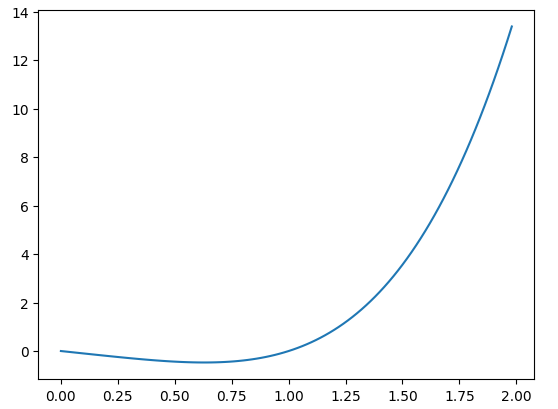
\includegraphics[width=6cm]{Imagenes/p3 ecuacion.png}
        \centering
    \end{figure}
Para este trabajo utilizamos un repositorio de GitHub con su aplicación para la maximización de funciones.\footcite{Dan20}
\framebreak

Generamos nuestra primera población:
    \begin{figure}[h]
       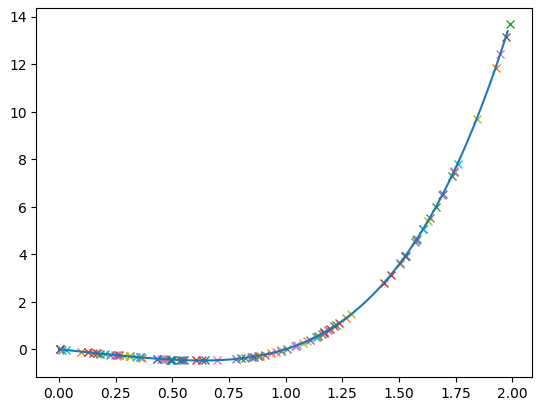
\includegraphics[width=6cm]{Imagenes/p3 1erag.png}
        \centering
    \end{figure}
A estos puntos los premiaremos cuando su valor sea mínimo y los castigaremos cuando el valor no cumpla con ese criterio, a esta evaluación se le conoce como "fitness"
\\
\framebreak
Luego de la primera generación, vemos que la distribución se ha movido ligeramente, pero no lo suficiente como para ser concluyente:
    \begin{figure}[h]
       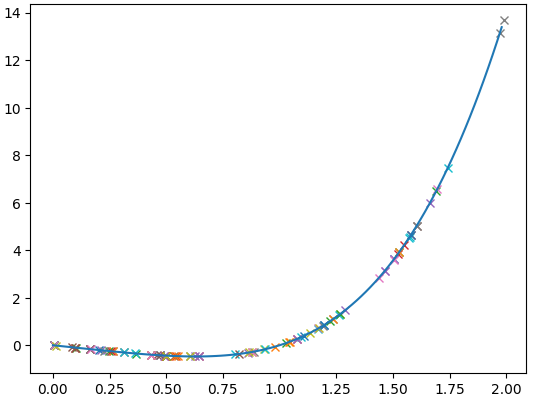
\includegraphics[width=6cm]{Imagenes/p3 2dag.png}
        \centering
    \end{figure}
Hay que resaltar que en todas las generaciones se aplicó una mutación, es decir, se vario uno de los genes de algunos individuos de manera aleatoria.
\\
\framebreak
Luego de 100 generaciones, la población se ha distribuido de la siguiente manera:
    \begin{figure}[h]
       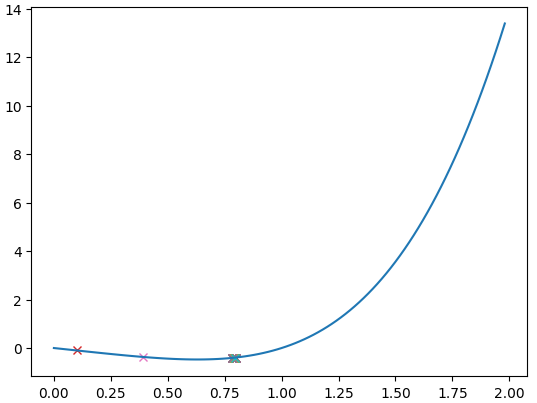
\includegraphics[width=6cm]{Imagenes/p3 100g.png}
        \centering
    \end{figure}
El valor de $x$ que arroja el mínimo en esta función ha sido $x=0.796$, un valor cercano al valor calculado, pero como hemos podido observar, luego de una determinada cantidad de generaciones, seguramente será posible obtener un valor más cercano al valor calculado analíticamente.
\\Si queremos seguir generando poblaciones, podemos utilizar el siguiente enlace hecho en Google Coolab para esta función: \href{https://colab.research.google.com/drive/1-Qyot1mxXB_5UUK7yPKAN7h3VYBSTotL#scrollTo=u9t-hjTo2aWS}{Enlace de Coolab}

\end{frame}
